\subsection{An actual signed-graph certificate at five thousand spins}
\label{sec:signed-memory-12}

The finite certificate now reaches the actual positive-fill
\texttt{signed\_packet} source at $N=5000$, inverse temperature $1/N$:
1000 disjoint negative pairs and 3000 correction-free sites on the dense
background, with ports $(0,1,60,61)$ and unit heatbath attempts per physical
site. Every microscopic flip is retained. This source is distinct from
the uniform complete-graph control and from its declared 16-mask boundary
heatbath.\samref{REF12_SPIN}

The source moments can be contracted without retrieving the terabyte
thermal archive. Conditioning on the observed pair leaves the factor
\begin{equation}
 (1+2e^{4/N}x+x^2)^{999}(1+x)^{3000},
\end{equation}
together with its retained common normalization and dense-field weights.
A positive degree-48 insertion expansion contracts the marked-pair and
free-site multiplicities, including the central rows, with a directed
tail payment. It is a static moment contraction of the actual generator
action, not a claim of dynamical lumpability of the pair counts.

For a stationary globally spin-flip-symmetric observation $S_t=\pm1$,
let $R(t)=\langle S_0S_t\rangle$. The exact three-time law at equal waits is
\begin{equation}
 p(s_0,s_1,s_2)=\tfrac18\{1+R(t)(s_0s_1+s_1s_2)
                              +R(2t)s_0s_2\}.
\label{eq:binary-three-law-12}
\end{equation}
Reversibility represents $R(t)$ as a Laplace transform of a positive
spectral measure. Positive Hankel moments give a two-node Gauss lower
and a left-zero Radau upper for this transform, with degenerate support
treated separately. Substitution into the positive-cell law, followed by
directed KL evaluation and its paid series remainder, certifies
\begin{equation}
 \begin{gathered}
 I(S_0;S_{2/3}\mid S_{1/3})\in
 [3.4208196027,\,3.4208514025]\\
 \times10^{-6}\ \mathrm{nats}.
 \end{gathered}
\label{eq:signed-cmi-12}
\end{equation}
The complete adjacent-correlation fit of every common scalar speed of
the declared four-port boundary heatbath gives
\begin{equation}
\begin{gathered}
 I_{\rm boundary}<7.678577136\,10^{-9}\ \mathrm{nats},\\
 I_{\rm micro}/I_{\rm boundary}>445.5017.
\end{gathered}
\end{equation}
This is stronger than the exploratory $445.4$ ratio. The fit, preparation,
ports and clock are part of the assertion; an arbitrary history-dependent
receiver is outside this fitted scalar family.

The later cross-volume refinement retains an additional
\texttt{signed\_packet\_chain} certificate
$[3.41219962633,3.41223131098]10^{-6}$ nats, recorded as TWO-F03.
Its original graph has 668 isolated pairs, 166 four-spin paths and 3000 free sites, with the observed pair untouched. It lies below the matching-source interval by about 0.2511--0.2529\%; adding bridges therefore does not monotonically increase this finite-lag information. It was not rerun in either H003005 or the present GEN7 window. Its status
and original source are retained separately in the evidence register.
The degree-48 four-spin chain insertion adapter in the earlier review
was preparation for this successor, not its completed numerical proof.
\samref{REF12_VOLIII}\samref{REF12_THREE}

\subsection{Uniform critical memory persists on growing waits}
\label{sec:growing-memory-12}

For the separate uniform positive-fill critical complete graph, put
$c_*=\sqrt{12}\,\Gamma(3/4)/\Gamma(1/4)$. On the original physical
attempt clock and for fixed $t_0>0$, the verified estimate is uniform on
$t_0\le t\le T_N=o(\sqrt N)$:
\begin{equation}
 \begin{split}
 I_{{\rm micro},N}(t)
 ={}&\frac{c_*^2\tanh^2(t/2)}{2N}\\
 &+O((1+t)N^{-3/2}+(1+t)^2N^{-2}).
 \end{split}
\label{eq:growing-memory-12}
\end{equation}
The derivation retains stationary quartic moments, the full Dirichlet
forcing estimate and lower-cell positivity before expanding the exact
binary law. It extends the fixed-wait $N^{-1}$ defect beyond a finite
thermal sweep. If additionally $t_N\to\infty$, then
$NI_N(t_N)\to c_*^2/2$; bounded waits retain the $\tanh^2(t/2)$ factor.
No divergent-wait limit follows from $t_N=o(\sqrt N)$ alone.

At $N=5000$, a fresh folded-source contraction including central
multiplicity gives
\begin{equation}
 I_N(4)\in[.0000970571116858,.0002503534522325]\ \mathrm{nats}.
\end{equation}
The lower is more than $22.08$ times the inherited wait-$1/3$ upper.
For independently prepared cycles of duration $2t$ it is more than
$1.84$ times as large per cycle time, even with the same nonnegative
preparation/readout overhead assigned to both cycles. These are certified
comparisons of two waits, not a global finite-source rate optimum or a
conversion to physical seconds.\samref{REF12_SPIN}

\begin{figure}[htbp]\centering
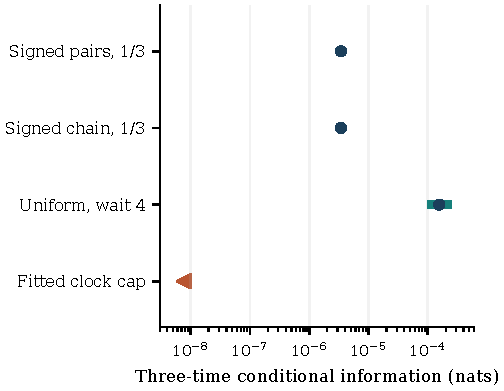
\includegraphics[width=\columnwidth]{refinement_20261112/figures/memory_certificates.pdf}
\caption{Directed information intervals for their stated source and
wait. The signed-source fitted-clock cap applies to its adjacent-
correlation-fitted boundary family. Wait four is a separate uniform-source
certificate. Bars distinguish models and preparations rather than pooling
them into one dynamical curve.}
\label{fig:memory-certificates-12}
\end{figure}
